\documentclass[tikz, preview]{standalone}

\usepackage{amsfonts, amsthm, amssymb, amsmath, stmaryrd, etoolbox}
\usepackage{tikz}
\usetikzlibrary{matrix,arrows}

\begin{document}
	\[
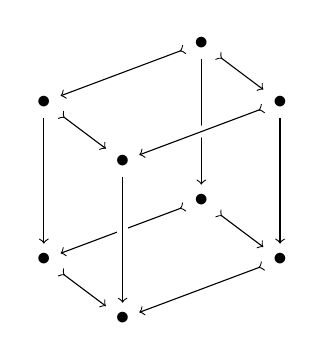
\begin{tikzpicture}
\node (tb) at (2,2.75) {$\bullet$};
\node (tl) at (0,2) {$\bullet$};
\node (tr) at (3,2) {$\bullet$};
\node (tf) at (1,1.25) {$\bullet$};
\node (bb) at (2,0.75) {$\bullet$};
\node (bl) at (0,0) {$\bullet$};
\node (br) at (3,0) {$\bullet$};
\node (bf) at (1,-.75) {$\bullet$};
%
\draw [>->] (tb) edge (tr);
\draw [->] (tb) edge (bb);
\draw [>->] (tb) edge (tl);
\draw [->] (tr) edge (br);
\draw [>->] (tl) edge (tf);
\draw [->] (tl) edge (bl);
\draw [>->] (bb) edge (br);
\draw [>->] (bb) edge (bl);
\draw [>->] (br) edge (bf);
\draw [>->] (bl) edge (bf);
%
\draw [->] (tf) edge[white,line width=4pt] (bf);
\draw [->] (tf) edge (bf);
\draw [>->] (tr) edge[white,line width=4pt] (tf);
\draw [>->] (tr) edge (tf);
\end{tikzpicture}
\]
\end{document}
